% Oppsett, ikke noe å bry seg om.
\documentclass[12pt,norsk,a4paper]{article}
\usepackage{graphicx}
\usepackage{hyperref}
\usepackage{float}
\usepackage{pdfpages}
\usepackage{ulem}
\usepackage[utf8]{inputenc}
\usepackage[norsk]{babel}
\usepackage{multirow}
\usepackage{colortbl}
\usepackage{array}

\begin{document}
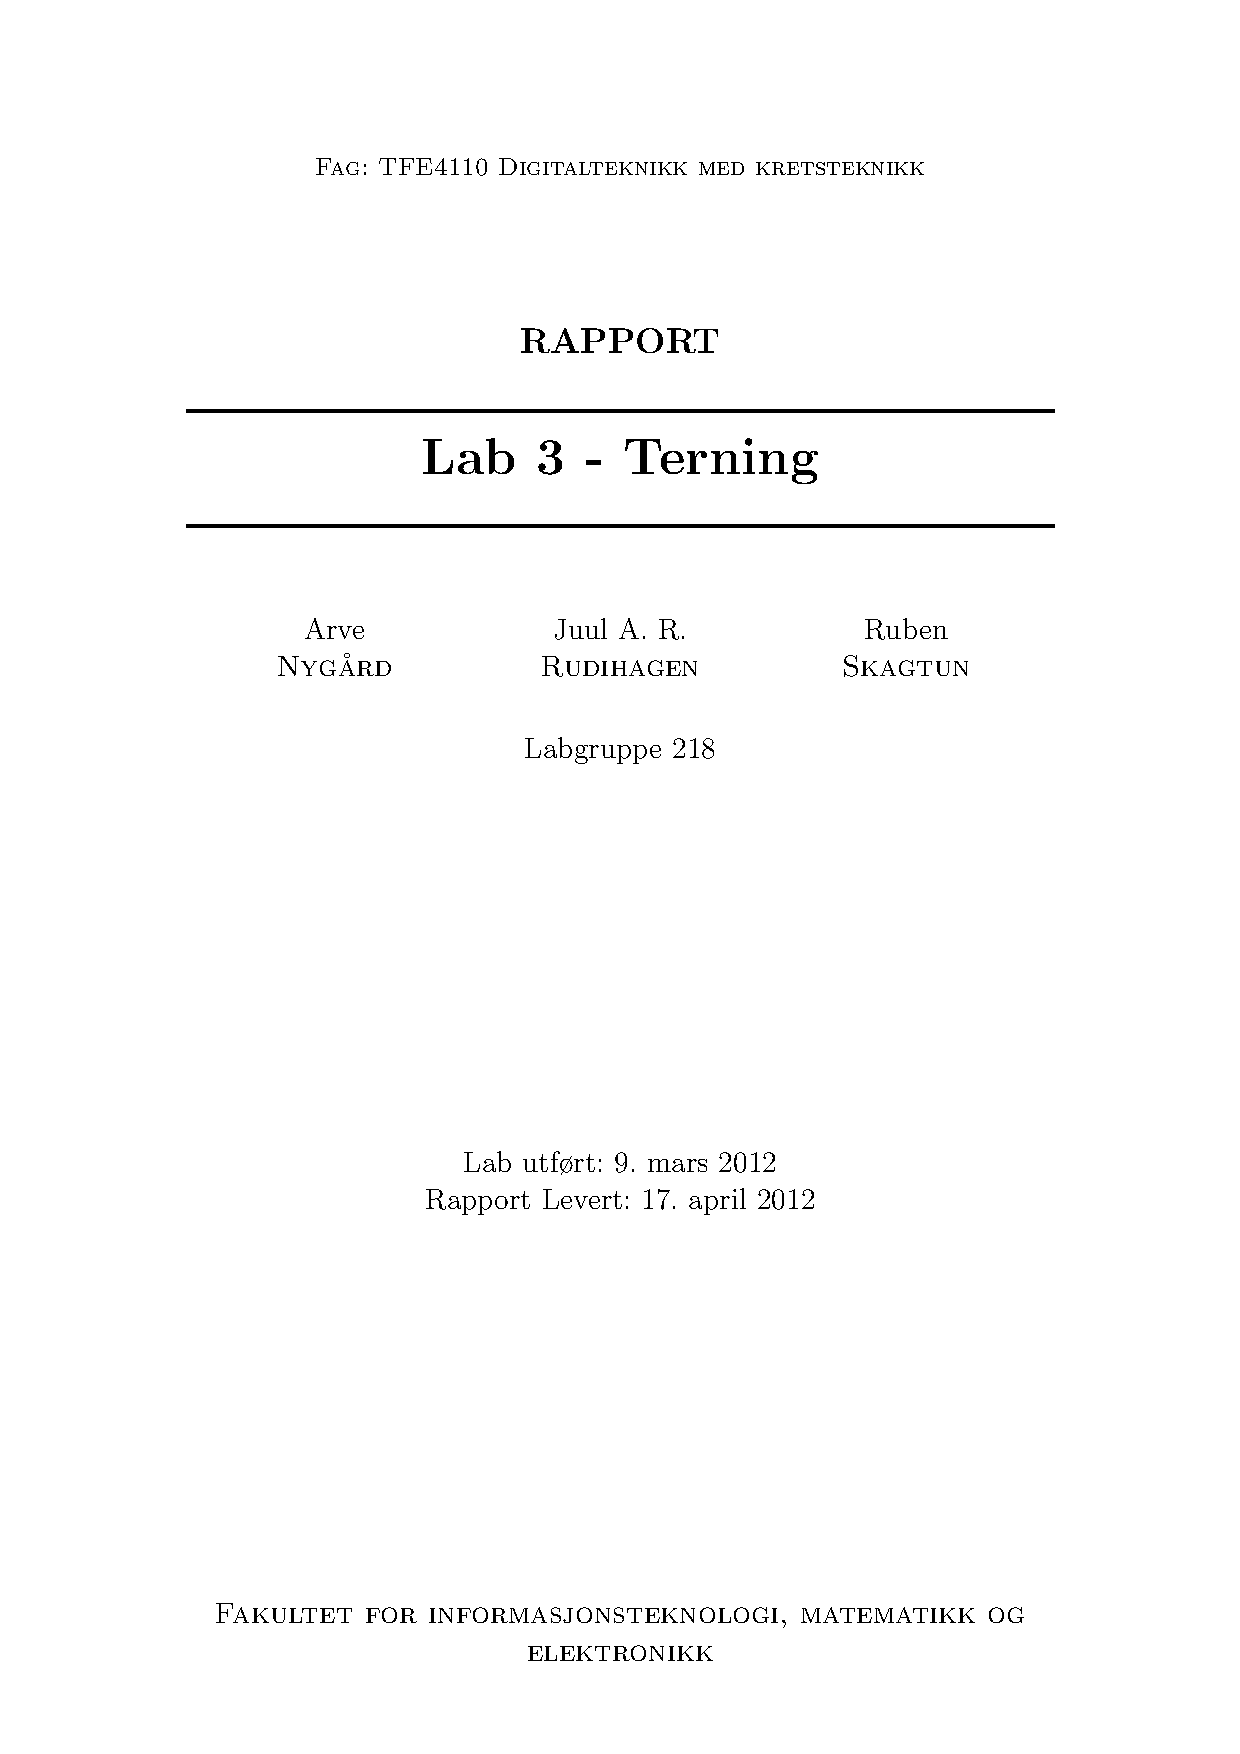
\includepdf{titlepage}
\clearpage



\section*{} % Stjerne etter section -> Siden tas ikke med når latex teller sidetall
\thispagestyle{empty}   
\begin{center}
\Large \textsc{Labrapport: Lab 3 - Terning}
\end{center}
\clearpage

\section*{Sammendrag}
\thispagestyle{empty}  

I denne rapporten blir det beskrevet hvordan gruppen utførte en laboppgave hvor målet var å lage en digital krets. Dette ble gjort ved hjelp av logiske portkretser som styrer lysdioder som igjen danner mønstrene til en vanlig sekssidet terning. Et viktig poeng er at terningen skal ha en uniform verdidistribusjon, slik at den oppfører seg som en virkelig terning.\\
\\
Etter å ha kommet frem til et design på papiret, ble kretsene loddet opp og testet. Gruppen fikk produsert to kretser som viste tilfeldige terningmønstre, som etter 60 testkjøringer viste seg å ha en uniform distribusjon av verdier. Et tredje kretskort ble startet på, men ikke fullført i tide.
\clearpage

\tableofcontents %Innholdsfortegnelse. Genereres automatisk. :)
\thispagestyle{empty}   
\clearpage

\section{Innledning} 
\setcounter{page}{1}
I dette eksperimentet skal gruppen designe, koble opp, og teste en digital krets som representerer en terning. Det skal først lages en skjematisk fremstilling av kretsen (fig. \ref{fig:kretskortet}), før denne loddes opp med fysiske komponenter. \\
\\
Terningen skal fungere på følgende måte: Du trykker ned en knapp for å rulle terningen. Når knappen er presset inn, vil tallgeneratoren rullere mellom verdiene 1-6, med svært høy hastighet. Når knappen slippes, stopper generatoren opp på nåværende tall, og vises ved hjelp av lysidodene. Det er kritisk at tallgeneratoren rullerer mellom verdier raskt nok til at det blir umulig for et menneske å forutsi hvilken verdi vil få.\\
\\
Terningen består av tre hoveddeler (fig. \ref{fig:blokkskjema}): En tilfeldig tallgenerator, logikk som konverterer tallet til et mønster, og lysdioder som viser dette mønsteret. Virkemåten til disse delene er forklart under teoridelen av rapporten.


\clearpage

\section{Teoretisk grunnlag}
Terningen består av tre hoveddeler: En tilfeldig tallgenerator som til enhver tid
gir ut et trebits binærtall mellom 1 og 6. Logikken skal så oversette denne tallrekken til et nytt firebits binærmønster som styrer lysdiodene. Til slutt viser lysdiodene et mønster som representerer tallet, slik som i en tradisjonell terning. Figur \ref{fig:blokkskjema} viser hvordan terningens hoveddeler henger sammen.

\begin{figure}[H]
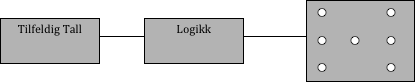
\includegraphics{Blokkskjema.png}
\caption{Hoveddelene til terningen}
\label{fig:blokkskjema}
\end{figure}

    \subsection{Tilfeldig tallgenerator}
    Den tilfeldige tallgeneratoren baser en teller som teller fra  001 og 110, som er henholdsvis 1 til 6 i en evig loop. Dette skjer vet at når telleren overstiger verdien seks begynner den å telle på en igjen. Telleren blir klokket av en oscillator som svinger
    veldig raskt, dette gjør at verdien til telleren skifter så fort at vi kan si det er tilfeldig hvilket tall som kommer ut når man slipper bryteren. Denne oscillatoren består av en NAND- og en NOR-port, i tillegg til noen motstander og kondensatorer.

    
    \subsection{Lysdioder}
    Lysdiodene på kretskortet som vi bruker til å vise hvilket tall terningen får er aktiv lave. Det vil si at dersom de får inn '0'
    så vil de lyse. Selv om dette kan virke forvirrende er det hensiktsmessig fordi det fører til at vi får mindre indre motstand. Dette fører igjen til at vi får mer strøm som gir sterkere lys. For å gi ut alle tallene en terning kan gi, ved en mest mulig lik tilnærming trenger vi 7 lysdioder og 4 styresignal. Grunnen til at vi bare trenger 4 styresignal til 7 lysdioder er fordi noen av dem kan kontroleres med samme styresignal (fig \ref{fig:terning}).

    \begin{figure}[H]
    \begin{center}
    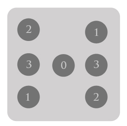
\includegraphics[scale=1]{Terning.png}
    \caption{Figur av terninen. Diodene med samme nummer lyser alltid samtidig}
    \label{fig:terning}
    \end{center}
    \end{figure}

    \subsection{Logikken}
    Logikken sin oppgave er å oversette signalene Q2-Q0 som representerer den binære verdien til hvilket tall terningen skal gi, til styresignalene S3-S0 som styrer lysene på terningen. Et poeng er å gjøre kretsen så effektiv som mulig, for å oppnå dette brukte vi Karnaugh-Diagram. Utledningen som ble gjørt er lagt ved som Vedlegg 1 og Vedlegg 2. En kort oppsumering av resultatet vises i tabellen under.\\

    \begin{table}[H] 
    \begin{center}
        \begin{tabular}{ | c | l |} 
        \hline
        $Styresignal$  & $Logisk uttrykk$ \\ \hline 
        S0 & $\neg Q_0$\\ \hline
        S1 & $\neg Q_2 \wedge \neg Q_1$\\ \hline
        S2 & $\neg Q_2$\\ \hline
        S3 & $\neg Q_2 + \neg Q_1$\\ \hline
        \hline
        \end{tabular}
        \end{center}
        \caption{Tabell på hvordan logikken konverterer ingangsbittene til styresignalene}

\end{table}
Ut fra denne tabellen kan vi sette opp hvordan den totale kretsen skal bli når vi kobler den sammen. Resultatet er fremstil på bilde under.

    \begin{figure}[H]
    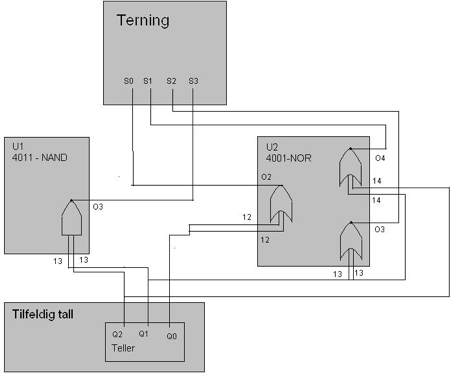
\includegraphics[scale=0.75]{Krestkortet.png}
    \caption{Sammenhengen mellom bitverdiene og styresignalende}
    \label{fig:kretskortet}
    \end{figure}
Som en ser på bilde har vi lagd inverterere ved å koble samme inngangsignal i begge inngangene på en NAND- eller NOR-port. Vi kunne oppnådd samme effekt dersom vi koblet en av inngangene til jord.   

\clearpage

\section{Målemetode og arbeidsbeskrivelse}
Forarbeidet til denne laboratorieøvelsen ledet gruppen frem til en komplett skjematisk fremmstilling av et kretskort som simulerer en terning. Selve laboratoriedelen besto av lodding og sammenkobling av tallgeneratoren, logikken og diodene.\\
\\
Det aller første gruppen måtte gjøre, var å lodde på alle komponentene på et av krestkortene. Dioder, IC-sokler, motstander osv., ble loddet på. Når dette var gjort, ble oscilloskopet brukt til å kontrollere at tallgeneratoren fungerte (se vedlegg 3). Alle prober på oscilloskopet ble kalibrert vha. oscilloskopets 'auto-check' funksjon. Tallgeneratoren ble deretter kontrollert vha. probene som var utgitt på labplassen. Målinger ble så tatt ved å holde proben inntil pinne 3 på $U_2$, samt $Q_2$, $Q_1$ og $Q_0$.\\
\\

Underveis i forsøket ble oscilloskopet også benyttet til å måle $S_0$ - $S_4$. Gruppen observerte at målingen med sannsynligheten for hvert signal når det er aktivt, stemte med utregningene som ble gjort i forarbeidet (tabell \ref{tbl:probe}).
\\
\\
Til slutt ble det utført 60 trykk på terningen. Dette ble gjort for å kontrollere at sannsynligheten til de forskjellige tallene tilfeldige. Resultatene er fremstilt i tabell \ref{tbl:probabilitetsdistribusjon}.
\clearpage


\section{Utstyrsliste} 
    \begin{itemize} 
    \item Kretskort

Serienummer: ZBX0512.169630-423
    \item Spenningskilde

Enhetsnummer: 74
    \item Plassnummer 47
    \item Multimeter

Enhetsnummer: 37
    \item Loddebolt

Enhetsnummer: 59
    \item Oscilloskop

Serienummer: G04-0281

    \end{itemize}
\clearpage


\section{Resultater}
Gruppen fikk ferdigstilt og testet to terningkretser. Det ble kontrollert at terningens output var normalt fordelt (tabell \ref{tbl:probabilitetsdistribusjon}, \ref{tbl:probe}).\\
\\Terningene er konstruert for å drives av en 5V spenningskilde, men gruppen rakk ikke å lage en batteriadapter. 


\begin{table}[H]
    \begin{center}
    \begin{tabular}{|c|c|}
    \hline
    Verdi & Antall ganger\\ \hline
    1 & 13 \\ \hline
    2 & 8  \\ \hline
    3 & 10 \\ \hline
    4 & 8  \\ \hline
    5 & 10 \\ \hline
    6 & 11 \\ \hline
    \end{tabular}
    \caption{Probabilitetsdistribusjon etter 60 'kast' på den første terningen.}
    \label{tbl:probabilitetsdistribusjon}
    \end{center}
    \end{table}
 \vspace{1cm}
\begin{table}[H]
    \begin{center}
    \begin{tabular}{|c|c|c|}
    \hline
    Pinne & $\frac{T_H}{T_D}$ (ms) & Probabilitet   \\[1mm] \hline
    $S_0$ & $\frac{1.13}{2.26}$  & $\frac{1}{2}$    \\[1mm] \hline
    $S_1$ & $\frac{1.13}{6.78}$  & $\frac{1}{6}$    \\[1mm] \hline
    $S_2$ & $\frac{3.39}{6.78}$  & $\frac{1}{2}$    \\[1mm]\hline
    $S_3$ & $\frac{5.65}{6.78}$  & $\frac{5}{6}$    \\[1mm] \hline
    \end{tabular}
    \caption{Probabilitetsdistribusjon for pinnene $S_0 - S_3$  på kretsen som styrer lysdiodene}
    \label{tbl:probe}
    \end{center}
    \end{table}

\clearpage

\section{Diskusjon}
Resultatet bekrefter at implementeringen er rett, de 60 kastene ble så jevnt fordelt som vi kunne forvente med så få kast. Vår analyse av utgangssignalene $S_0 - S_3$ (tabell \ref{tbl:probe})ble akkurat som forventet ut ifra forarbeidet. Som en kan se i tabell [\ref{tbl:probabilitetsdistribusjon}], fikk vi alle kombinasjoner av øyne som en terning kan gi, og ingen ulovlige verdier. Vi anser det som at implementeringen av terningen var vellykket, og at det ikke er noen defekte deler eller feil i logikken. 


\clearpage

\section{Konklusjon}
Gruppen konkluder med at det med god planlegging og godt forarbeid lar seg gjøre å bruke logiske kretser til å lage en digital terning. Man kan se at det er mulig å simulere en tilfeldig tallgenerator ved å traversere gjennom et intervall, så lenge frekvensen er høy nok til at et menneske umulig kan forutsi resultatet. \\
\\
For å kunne konkludere med høyere sikkerhet at terningen er riktig implementert burde vi testet med flere enn 60 forsøk at terningen gav en jevn fordeling av verdier. Men ut ifra de testene vi gjorde var resultatet lovende. \\
\\
Alt i alt kan vi konkludere at med den enkle teorien som er brukt i oppgaven kan vi lage et reelt produkt som fungerer. 

\clearpage

\section{Vedlegg}
    \subsection{Vedlegg 1: sammenheng mellom binærverdi og styresignal.}
    \begin{table}[H]
    \begin{center}
    \begin{tabular}{|c|c|c|c|c|c|c|c|c|}
    \hline
    Hex & \multicolumn{3}{c}{Binærverdi} & \multicolumn{4}{|c|}{Styresignal}&hex \\ \hline
    $Q$ & $Q_2$ & $Q_1$ & $Q_0$ & $S_3$ & $S_2$ & $S_1$ & $S_0$ & $S$ \\ \hline
    0 & 0 & 0 & 0 & X & X & X & X & - \\ \hline 
    1 & 0 & 0 & 1 & 1 & 1 & 1 & 0 & E \\ \hline
    2 & 0 & 1 & 0 & 1 & 1 & 0 & 1 & D \\ \hline
    3 & 0 & 1 & 1 & 1 & 1 & 0 & 0 & C \\ \hline
    4 & 1 & 0 & 0 & 1 & 0 & 0 & 1 & 9 \\ \hline
    5 & 1 & 0 & 1 & 1 & 0 & 0 & 0 & 8 \\ \hline
    6 & 1 & 1 & 0 & 0 & 0 & 0 & 1 & 1 \\ \hline
    7 & 1 & 1 & 1 & X & X & X & X & - \\ \hline
    \end{tabular}
    \end{center}
    \caption{Resultat $S_0=\neg Q_0$}
    \end{table}
    \clearpage

    \subsection{Vedlegg 2: Karnaugh-Diagram}
    \begin{table}[H]
    \begin{center}
    \begin{tabular}{|l|l|r|r|} \hline
    \multicolumn{4}{|c|}{Tabell for $S_0$} \\ \hline
    $Q_2$ & $Q_1$ & \multicolumn{2}{|r|}{$Q_0$ \hspace{20 mm} 0 \hspace{2 mm} 1} \\ \hline
    0 & 0 & \hspace{27 mm} X \cellcolor[gray]{0.8} & 0 \\ \hline 
    0 & 1 & 1 \cellcolor[gray]{0.8} & 0 \\ \hline
    1 & 1 & 1 \cellcolor[gray]{0.8} & X \\ \hline
    1 & 0 & 1 \cellcolor[gray]{0.8} & 0 \\ \hline
    \end{tabular}
    \end{center}
    \label{juul}
    \caption{Resultat $S_0=\neg Q_0$}
    \end{table}

    \begin{table}[H]
    \begin{center}
    \begin{tabular}{|l|l|r|r|} \hline
    \multicolumn{4}{|c|}{Tabell for $S_1$} \\ \hline
    $Q_2$ & $Q_1$ & \multicolumn{2}{|r|}{$Q_0$ \hspace{20 mm} 0 \hspace{2 mm} 1} \\ \hline
    0 & 0 & \hspace{27 mm} X \cellcolor[gray]{0.8} & \cellcolor[gray]{0.8} 1 \\ \hline 
    0 & 1 & 0 & 0 \\ \hline
    1 & 1 & 0 & X \\ \hline
    1 & 0 & 0 & 0 \\ \hline
    \end{tabular}
    \end{center}
    \caption{Resultat $S_1=\neg Q_2 \wedge \neg Q_1$}
    \end{table}


    \begin{table}[H]
    \begin{center}
    \begin{tabular}{|l|l|r|r|} \hline
    \multicolumn{4}{|c|}{Tabell for $S_2$} \\ \hline
    $Q_2$ & $Q_1$ & \multicolumn{2}{|r|}{$Q_0$ \hspace{20 mm} 0 \hspace{2 mm} 1} \\ \hline
    0 & 0 & \hspace{27 mm} X \cellcolor[gray]{0.8} & \cellcolor[gray]{0.8} 1 \\ \hline 
    0 & 1 & 1 \cellcolor[gray]{0.8} & 1 \cellcolor[gray]{0.8} \\ \hline
    1 & 1 & 0 & X \\ \hline
    1 & 0 & 0 & 0 \\ \hline
    \end{tabular}
    \end{center}
    \caption{Resultat $S_2=\neg Q_2$}
    \end{table}

    \begin{table}[H]
    \begin{center}
    \begin{tabular}{|l|l|r|r|} \hline
    \multicolumn{4}{|c|}{Tabell for $S_0$} \\ \hline
    $Q_2$ & $Q_1$ & \multicolumn{2}{|r|}{$Q_0$ \hspace{20 mm} 0 \hspace{2 mm} 1} \\ \hline
    0 & 0 & \hspace{27 mm} X \cellcolor[gray]{0.8} & \cellcolor[gray]{0.8} 1 \\ \hline 
    0 & 1 & 1 \cellcolor[gray]{0.8} & 1 \cellcolor[gray]{0.8} \\ \hline
    1 & 1 & 0 & X \\ \hline
    1 & 0 & 1 \cellcolor[gray]{0.8} & 1 \cellcolor[gray]{0.8} \\ \hline
    \end{tabular}
    \end{center}
    \caption{Resultat $S_3=\neg Q_2 + \neg Q_1$}
    \end{table}
\clearpage

    \subsection{Vedlegg 3: Oscillatorbilder}
    \begin{figure}[H]
    \begin{center}
    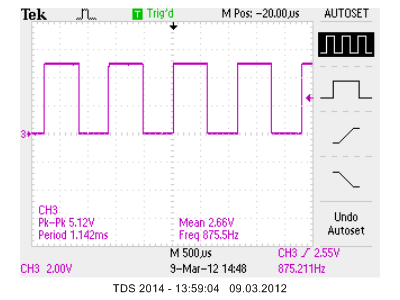
\includegraphics[scale=1.0]{Fig1.png}
    \caption{Oscillatorfrekvens målt på pinne 3 på U2.}
    \end{center}
    \label{fig:Oscillatorbilde1}
    \end{figure}

    \begin{figure}[H]
    \begin{center}
    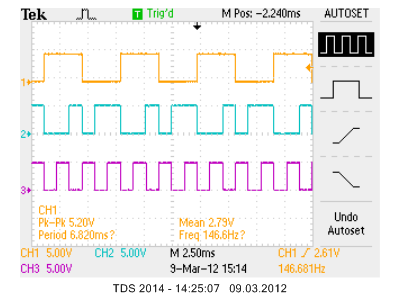
\includegraphics[scale=1.0]{Fig2.png}
    \caption{Måling med probene Q2, Q1 og Q0.}
    \end{center}
    \label{fig:Oscillatorbilde2}
    \end{figure}


\clearpage

\section{Litteraturhenvisninger}
$[1]$ Hergum \& Helland \& Hansen \textit{TFE4110 Digitalteknikk med kretsteknikk - Laboratoriehefte - Vår 2012} \\
\\
$[2]$ Daniel D. Gajski \& Prentice Hall: \textit{Principles of Digital Design US ed.} (Pearson US Imports \& PHIPEs, 1996) \\ %Mulighet for å få inn & istedet for AND?
\\

\clearpage

\section{Tilbakemeldinger}
Det hadde vært kjekt om det var klargjort batteriadapter til denne oppgaven. Enten bare en ferdiglaget adapter, eller at dette ble tatt med som en del av oppgaven. Kanskje designet av en kunne vært med som forhåndsoppgave.\\
\\
Ellers synes alle på gruppen at dette var en morsom lab! Kjekt å få med seg en selvprodusert digital terning hjem!
\clearpage
\end{document}